\documentclass[../main.tex]{subfiles}

\begin{document}

\subsection{Library}
As we mentioned before, as part of our effort to create a data collection system for our project,
 we created a library that could handle the data collection independently of the user interface or even the type of data. 
 The library is essentially a runtime meant to run on the user's computer and allows different data types to be collected. 
 The library exposes a simple API that enables users to implement their data collection, 
 processing, and saving mechanisms and provides the data collection and processing we needed for our project. Following is a description of 
 the functionality the library provides: 

 \begin{itemize}
    \item We provide a generic data collector class that 	can be loaded into the runtime:
        \begin{lstlisting}[language=Python]
        class DataCollector(ABC):

            def __init__(self):
                self.collect = True
                self.data = list()

            @abstractmethod
            def start_collect(self):
                ...

            @abstractmethod
            def stop_collect(self):
                ...
        \end{lstlisting}
        This class should implement the start and stop collect methods and save the data into the \textit{self.data} varialbe where
        the runtime will be able to use it for the processing step.
    \item We provide a generic data processor that the runtime provides with the data collected in the collector at the end of each session (discussed later):
        \begin{lstlisting}[language=Python]
            class DataProcessor(ABC):

                def __init__(self):
                    super().__init__()
                    self.features = None

                @abstractmethod
                def process_data(self, data, session):
                    ...
        \end{lstlisting}

        This class shoud implement the \textit{process\_data} method, receiving the data from the collector, and session object. This mehod should not take a long time
        to execute as it runs between sessions and taking too long could distrupt the data collection process. The runtime shoud not exceed one second, thouth this 
        is hard to verify due to users having different hardware. By the end of the processing the resulting features should be se into the \textit{self.features} object 
        as a map of $name \leftarrow feature$.
    \item We provide an abstraction over data preseistance in order to allow users to save the collected data in any way they choose:
        \begin{lstlisting}[language=Python]
            class DataHandler(ABC):

                def __init__(self, path):
                    super().__init__()
                    self.path = path

                @abstractmethod
                def save(self, data):
                    ...

                @abstractmethod
                def create_data_holder(self, i=-1):
                    ...

            class DatabaseManager(DataHandler):

                def __init__(self, path):
                    super().__init__(path)
                    self.path = path
            
                def save(self, data):
                    ...
            
                @abstractmethod
                def save_session(self, session):
                    ...
            
                @abstractmethod
                def create_data_holder(self, i=-1):
                    ...
            
                @abstractmethod
                def ask(self, query):
                    ...
            
                @abstractmethod
                def __len__(self):
                    ...
            
        \end{lstlisting}
        The user should implement two classes to specify a custom destination for the data. The user should implement the \textit{DatabaseManager} 
        class once for each data destination. For example, if we would like to save the data into a local SQLite database and a remote PostgreSQL server, 
        we will need to implement the class once for SQLite and once for PostgreSQL. 
        The user would need to implement \textit{ask} to send a query to the appropriate database and return the result.
        The \textit{save\_session} method should implement the saving of a session object to the database.
        The \textit{create\_data\_holder} method is called by the runtime on initialization and should create the database/table required to save the session later.
        Finally, the $\_\_len\_\_$ method should return the number of sessions held in the database. 
        The \textit{DataHandler} class should be implemented for each type of data that needs to be saved, here the \textit{save} method should handle the 
        saving of the data that came from the processor, and the \textit{create\_data\_holder} should create the table/collection where the data needs to be saved.
    
    \begin{figure}[htp]
        \centering
        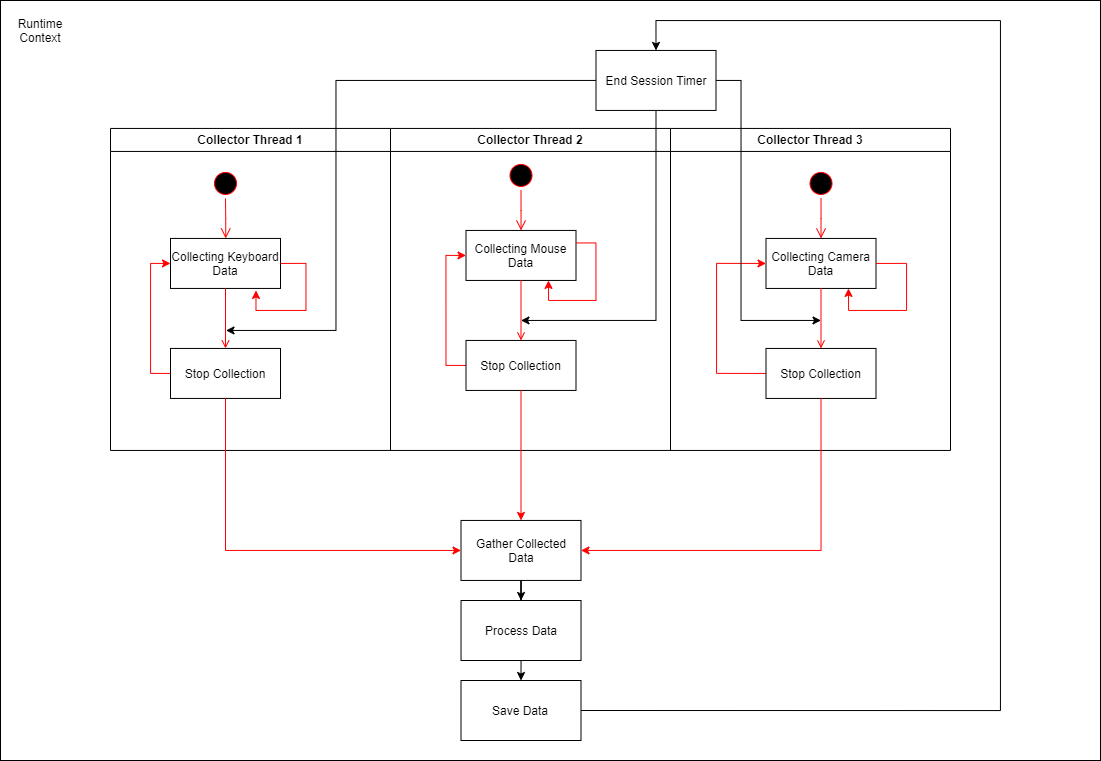
\includegraphics[width=14cm]{figures/sys_activity}   
        \caption{Activity diagram describing the session loop in our system.}
        \label{fig:sys_activity} 
    \end{figure}


    In \ref{fig:sys_activity} we can see the main loop of our runtime. We gave as an example here the collection methods that we ended up using in 
    our project. Still, the Collector threads can run any class that implements the \textit{DataCollector} class as described above. 
    When initializing the runtime, the user can specify the session length, and the End Session Timer will notify the collector threads to 
    stop collecting at the end of each session. Once the collection threads are notified, all the collected data is aggregated, and we run the 
    processor and finally save the data and start the next session. For every number of sessions, the system will need to ask the user for labels. 
    The user of this library implements the mechanism for labeling. We will discuss our implementation in the following sections.


    To coordinate, which collector needs to pass its data to what processor and where the processor needs to save its data, 
    our init method accepts a graph of collectors, processors, and data handlers that the runtime will use as a dictionary. 
    The graph is represented by a dictionary that contains the direction of data flow. For example, 
    if we want the mouse collector to pass its data to the mouse processor and a unit processor, and finally save all the data into the SQLlite data handler. 
    We would need to pass a dictionary that looks like the following:
    MouseCollector(): \{ MouseProcessor(): [MouseDataHandler(self.out\_path)], IdentityProcessor(): [RawDataHandler("MouseRawData", self.out\_path)] \}

 \end{itemize}

\subsection{Application}


Here we describe the structure of the application we used to collect data in our experiments, built on top of the library described above. 
Our application is separated into a \textit{Backend} and \textit{Frontend}. Both run on the same computer in our case. 
The backend uses our library to collect data from the user, and the frontend is the GUI we built for the user interaction.

\subsubsection{Backend}
As mentioned above, the backend uses our library to collect data. We use the default for collection, processing, and saving the data. 
The data we collect is from the mouse, keyboard, and camera if available. Our backend also implements the labeling mechanism, 
which prompts the user for a label every constant amount of time, one minute in our experiments.
The bolk of the backend is the communication with the frontend. Here we can see all the message types passed between them:

\begin{itemize}
    \item Close Connection - message sent from the GUI to the backend to indicate that a connection is no longer required and the backend can shutdown.
    \item Download Face Model - message sent from the GUI to downloads the dlib model we use for preprocessing.
    \item Download Task keywords - message sent from the GUI to downlaods the mapping we created form window type to task type.
    \item Run Core - message sent from the GUI to start the collection process.
    \item Stop Core - message sent from the GUI to stop the collection process.
    \item Label - message sent from the GUI containing a label from the user.
    \item Request label - message sent from the Backend when it needs a label.
    \item Core Finished - message sent from the Backend when the backend has finished collecting data
    \item Unknown - any other messages that are not specefied above are included here usually just to be logged.
\end{itemize}

\subsubsection{Frontend}

We used electron with Vue as the frontend framework to write our user interface. 
The application does not have many features. We have four main pages in the application:

\begin{itemize}
    \item Home Page \ref{fig:ui_home} - here we show some system statistics such as RAM CPU and Disk usage to allow the user to notice quickly if the system is 
        doing something odd. When the collection process is running, we also show the runtime since the user started collecting data.
        The time until the system will request the next label, and the current mood of the user (according to what was specified in the last label).
    \item Label Page \ref{fig:ui_label} - the user is prompted with this page whenever the backend requests a label, and the user can specify how he is feeling and submit the from.
    \item About Page \ref{fig:ui_about} - some basic information about who we are, what kind of data we collect, and what we will do with it.
    \item Settings Page \ref{fig:ui_settings} - some basic settings for our application such as, what collectors should be used, what the labeling frequency should be, what 
        the session duration should be and how many sessions the application should collect.
        We set the number of sessions to -1 by default to indicate that the system will keep running until the user stops it.

\end{itemize}

Finally we also have a start/stop button on the top right of the window available to easily start or stop the collection process.

\begin{figure}[htp]
    \centering
    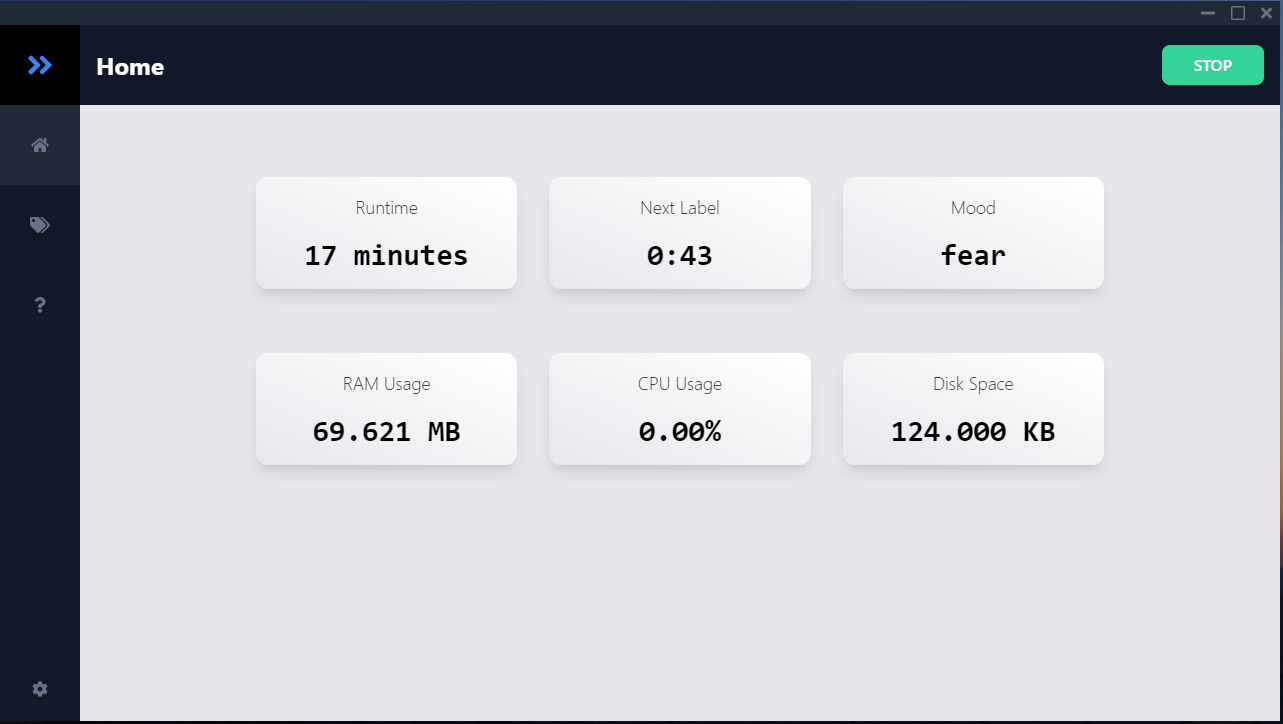
\includegraphics[width=14cm]{figures/ui_home}   
    \caption{Image of the GUI of out data collection application.}
    \label{fig:ui_home} 
\end{figure}

\begin{figure}[htp]
    \centering
    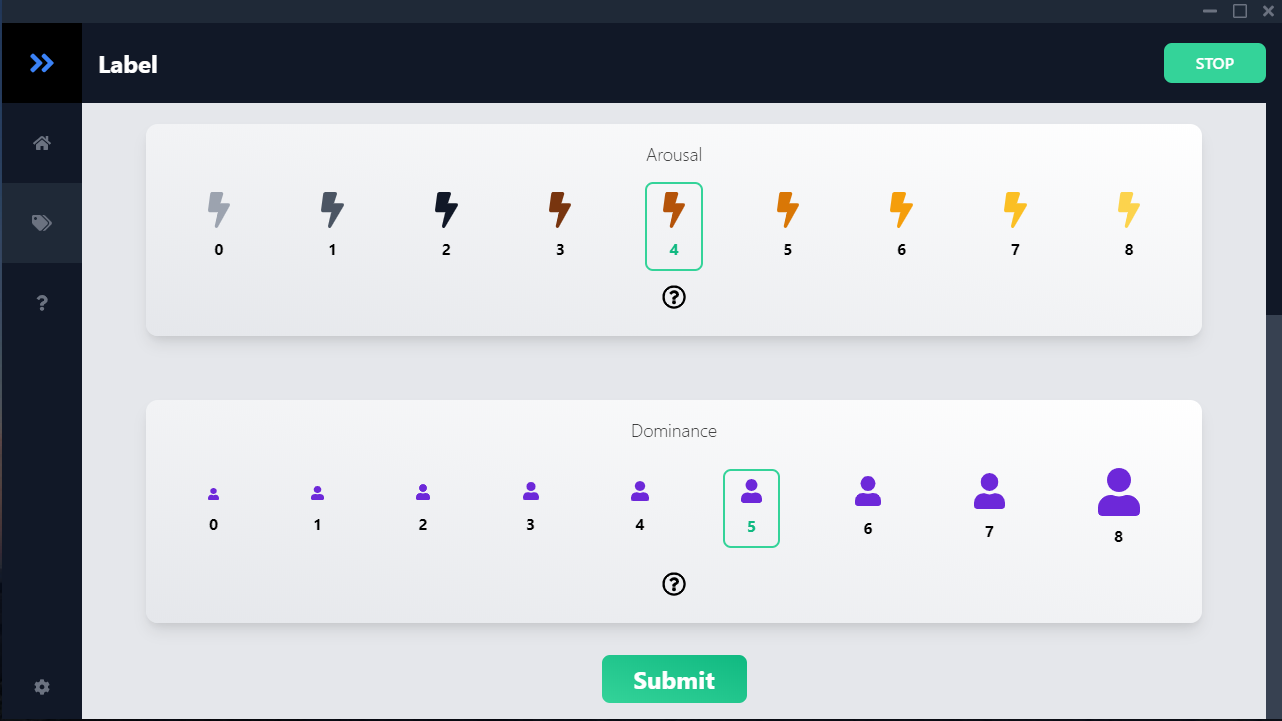
\includegraphics[width=14cm]{figures/ui_label}   
    \caption{Image of the GUI of out data collection application.}
    \label{fig:ui_label} 
\end{figure}

\begin{figure}[htp]
    \centering
    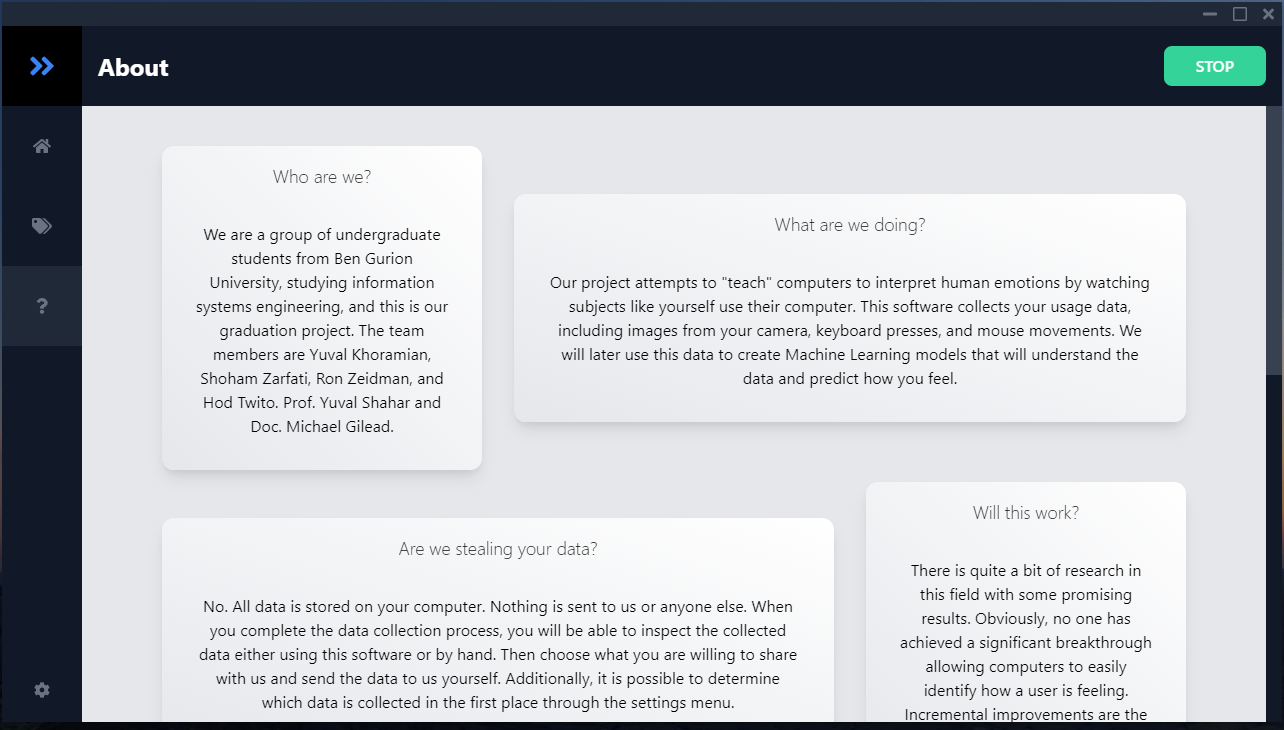
\includegraphics[width=14cm]{figures/ui_about}   
    \caption{Activity diagram describing the session loop in our system.}
    \label{fig:ui_about} 
\end{figure}

\begin{figure}[htp]
    \centering
    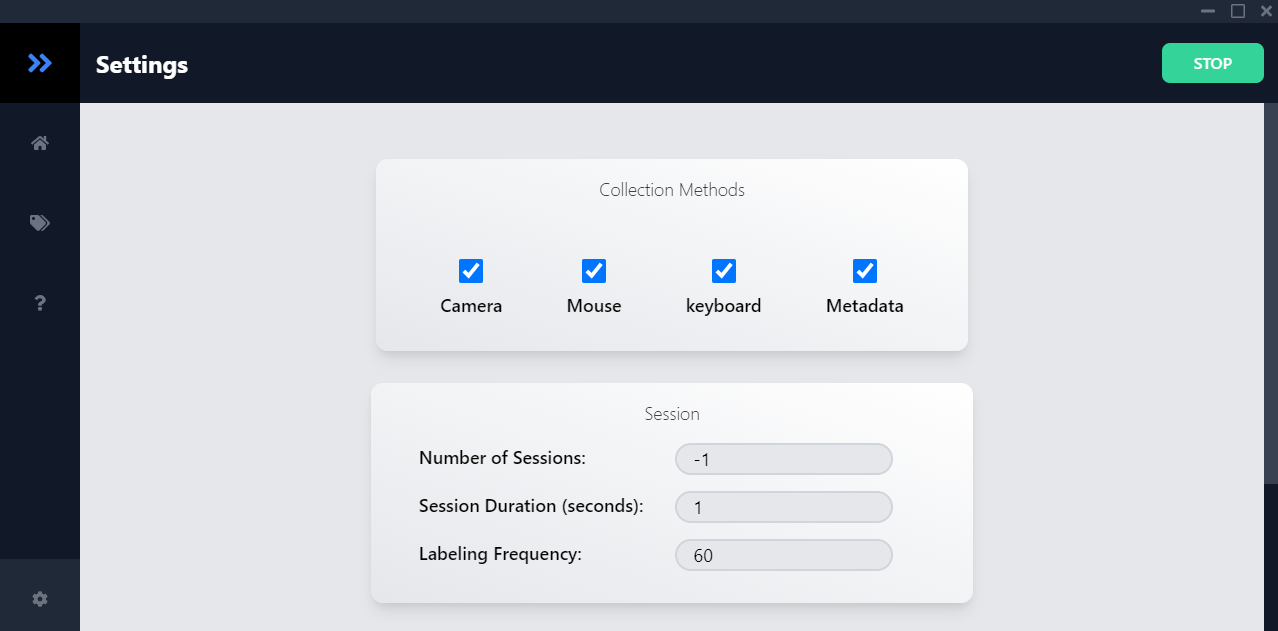
\includegraphics[width=14cm]{figures/ui_settings}   
    \caption{Activity diagram describing the session loop in our system.}
    \label{fig:ui_settings} 
\end{figure}

\end{document}
